\documentclass[12pt]{beamer}
\usetheme{CambridgeUS}
\usecolortheme{beaver}
%\usetheme{diepen}
%\usecolortheme{wolverine}
%\setbeamertemplate{background canvas}[vertical shading][top=magenta!15,bottom=cyan!20]
\documentclass{beamer}
\setbeamertemplate{background}{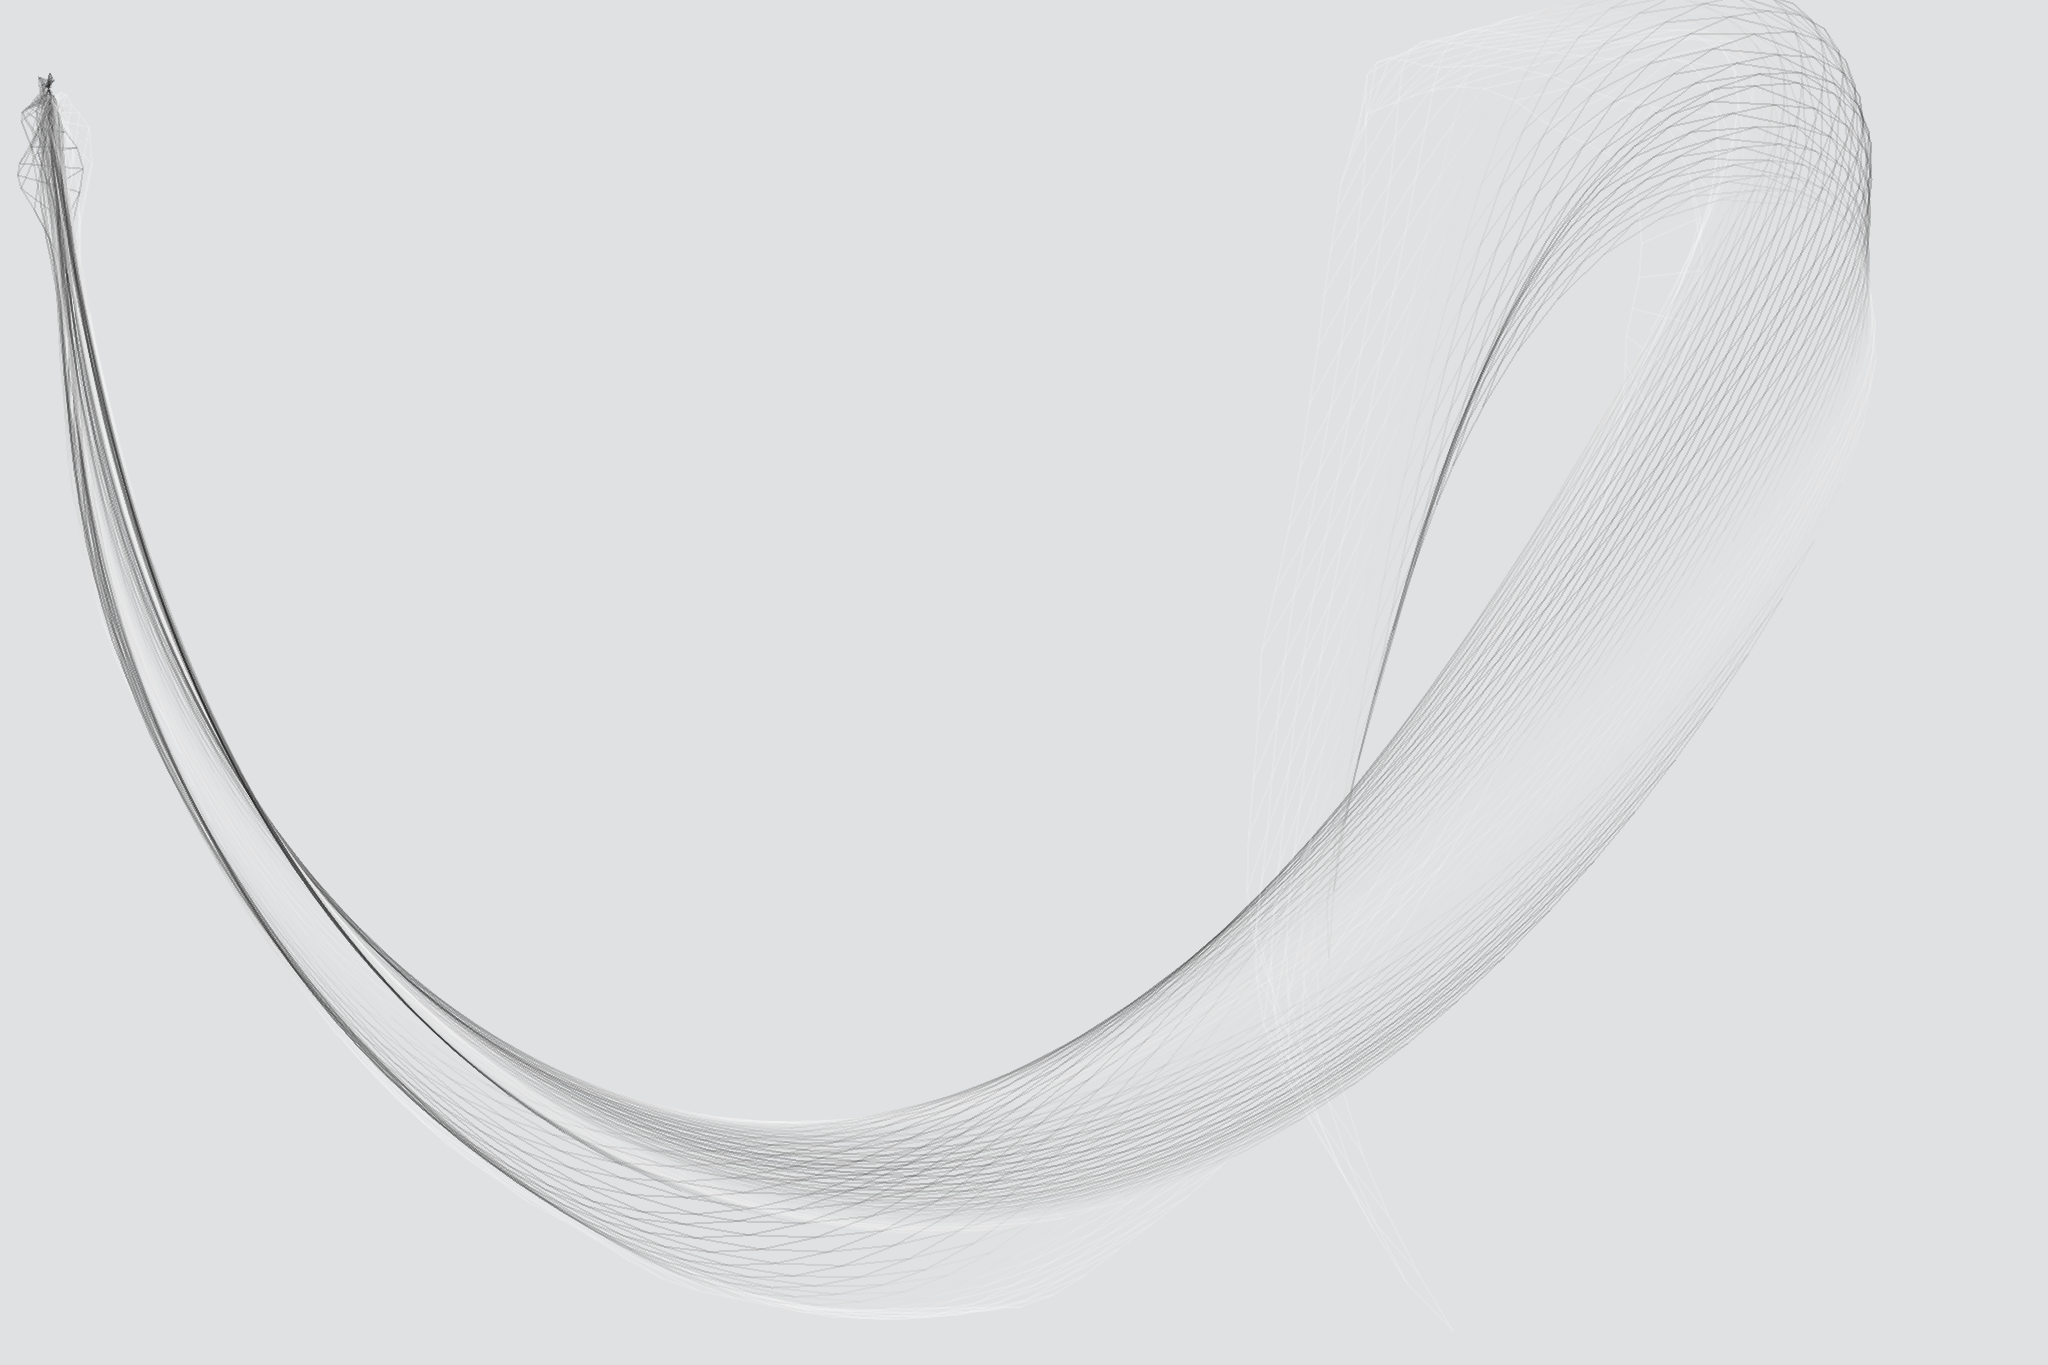
\includegraphics[width=\paperwidth,height=\paperheight]{1234567}}




\setbeamercolor{block title example}{bg=pink}
\usepackage{url}
\usepackage{chapterbib}
\usepackage{hyperref} 

 \usepackage{multicol}
% \usepackage{pgf,pgfarrows,pgfnodes}
% \usepackage{verbatim} 
%\usepackage{comment}
%\usepackage{multirow}
% \usepackage{graphics}
% \usepackage{graphicx}
% \usepackage{tikz}
%\usepackage{pgfplots}
%Basic Information
%\renewcommand{\bibname}{References}

\title{Aadhar Authentication for Aakash Tablet}




% \column{0.32\textwidth}
% Archana Iyer\\
% Hitesh Yadav\\
% Pooja Deo\\
% Prashant Main\\
% Prateek Somani\\[12pt]
% Prathamesh Paleyekar\\
% Sonu Philip\\
% Sudhanshu Verma\\
% \column{0.72\textwidth}
% Dwarkadas J. Sanghvi College of Engineering\\
% Visvesvaraya National Institute of Technology\\
% Visvesvaraya National Institute of Technology\\
% Terna Engineering College\\
% Bhagwan Mahavir College of Engineering and Technology\\
% Visvesvaraya National Institute of Technology\\
% National Institute of Technology Calicut\\
% Visvesvaraya National Institute of Technology\\
% \end{columns}


\author{Archana Iyer\hskip60pt D. J. S. \\Hitesh Yadav\hskip60pt VNIT \\ Pooja Deo \hskip60pt VNIT \\Prashant Main \hskip50pt Terna Eng.\\Prateek Somani \hskip60pt B. M. Eng. \\Prathamesh Palyekar \hskip20pt VNIT \\Sonu Philip \hskip60pt NIT-C \\Sudhanshu Verma \hskip40pt VNIT }
% 

%\author{Archana Iyer \\Hitesh Yadav \\Pooja Deo\\Prashant Main\\Prateek Somani \\Prathamesh Paleyekar\\Sonu Philip\\Sudhanshu Verma}
%\institute{Dwarkadas J. Sanghvi College of Engineering\\Visvesvaraya National Institute of Technology\\Terna Engineering College\\Bhagwan Mahavir College of Engineering and Technology\\National Institute of Technology Calicut}
\date{\vskip-20pt 03 July 2013}

\begin{document}
\begin{frame}

\titlepage
\vskip-20pt
 
\includegraphics[width=1cm]{./dj.jpg}
\hfill
 
\includegraphics[width=1cm]{./nitc.jpg}
\hfill
 
\includegraphics[width=1cm]{./t.jpg}
\hfill
 
\includegraphics[width=1cm]{./vnit.jpg}
\hfill
 
\includegraphics[width=1cm]{./111.jpg}

 \end{frame}

\begin{frame}
\frametitle{Outline}
\begin{multicols}{2}
\tableofcontents
%\tableofcontents[hideallsubsections]
\end{multicols}
\end{frame}

\section{Scope}
\begin{frame}[c]
\frametitle{Scope}

\begin{enumerate}
\item The project is focused primarily on capturing the user’s fingerprint using Aakash tablet.
\item The existing system uses an external scanner. This makes it expensive. The system developed by the team uses an optical assembly which makes use of the Aakash tablet’s camera. Hence it is cost effective.
\item The image thus captured is refined and sent to the Authentication Service Agency(ASA) server for the authentication of the Aadhar card holder. 
\end{enumerate}
\end{frame}


\section{Existing Product}
\begin{frame}[c]
\frametitle{Existing Product}
\begin{enumerate}
\item Provided by Futronic tech.
\item Costs around Rs.4000.
\item Can be connected to the tablet with the help of OTG cable and requires drivers  software.
\item Has a high-end camera.
\item Uses Infrared lightning.
\end{enumerate}
\begin{figure}
 \centering
 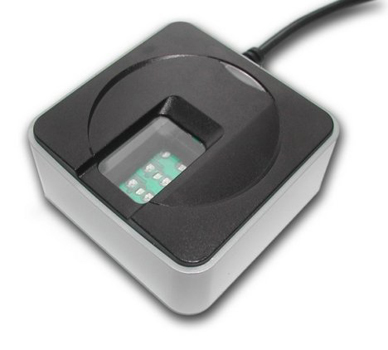
\includegraphics[width=3.8cm]{./ft.jpg}
 \caption{1.Futronic Tech Device}
\end{figure}
 \end{frame}


\section{Optical assembly}
\begin{frame}[c]
\frametitle{Optical assembly}
\begin{figure}
 \centering
 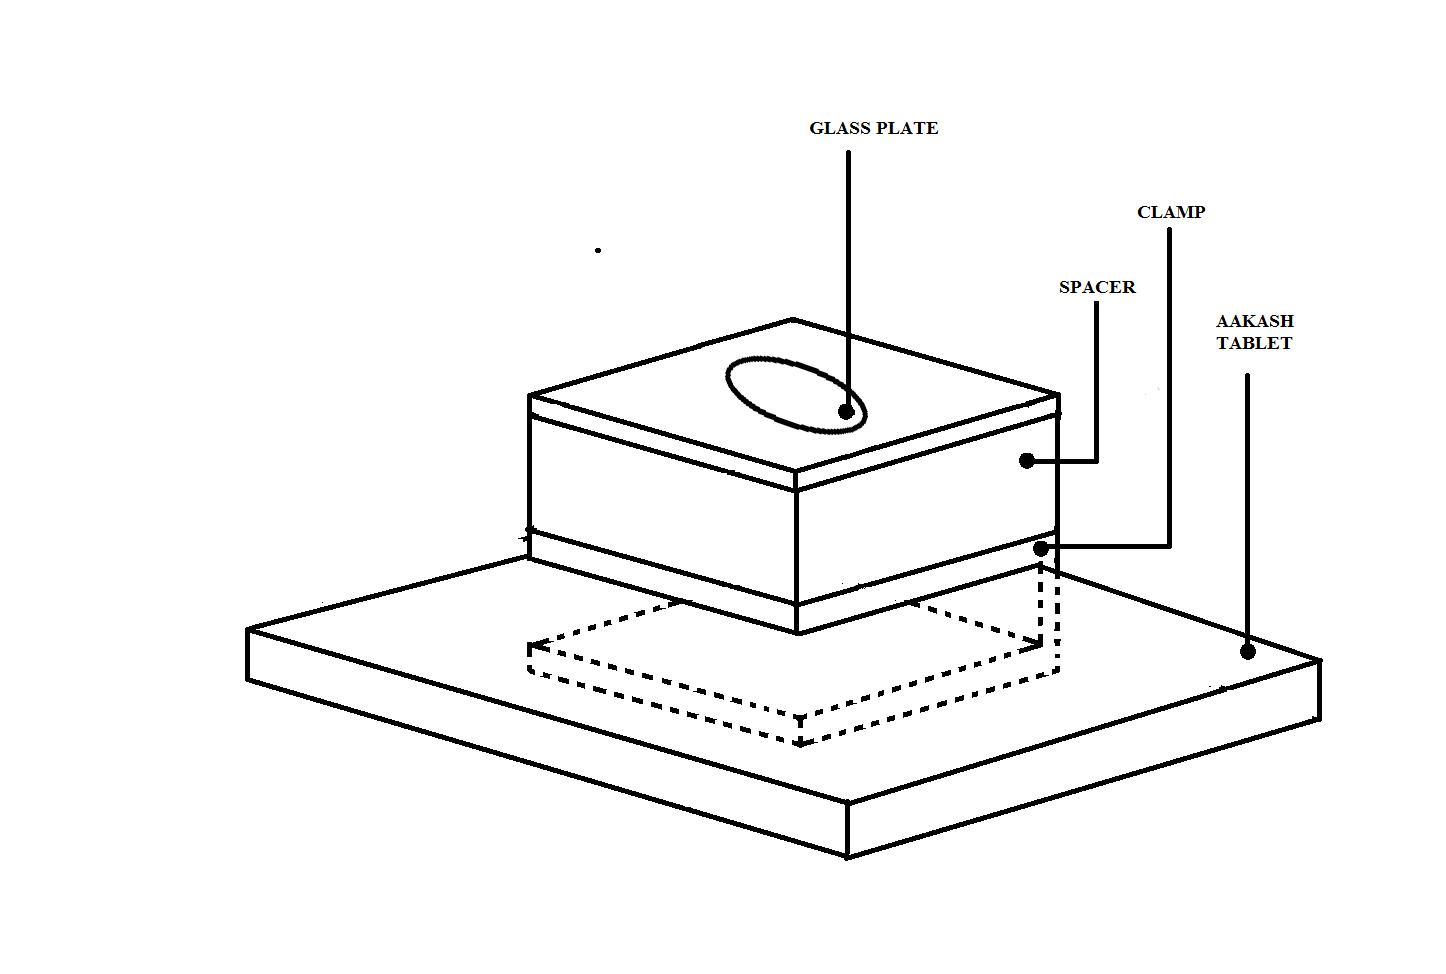
\includegraphics[width=10cm]{./oa.jpg}
 \caption{2.Optical Assembly}
\end{figure}
\end{frame}

\section{Components of optical assembly}
\begin{frame}[c]
\frametitle{Components of optical assembly}
\begin{enumerate}

\item \vskip-20pt Clamp: The clamp is built to fix the assembly to the tablet over the camera
\item Spacer:  A predefined distance needs to be maintained between the finger and the camera in order to obtain a clear image.The spacer undertakes this functionality. 
\item Optics: This assembly works on the FTIR principle (Frustrated total internal reflection). 
\begin{itemize}
\item PCB(Printed Circuit Board)
\item Lid
\end{itemize}
\end{enumerate}
\end{frame}




%--------------------------------------------------------------------------------------
%               Slide 4
%--------------------------------------------------------------------------------------
\section{}
\begin{frame}[c]
\frametitle{}
\begin{figure}
 \centering
 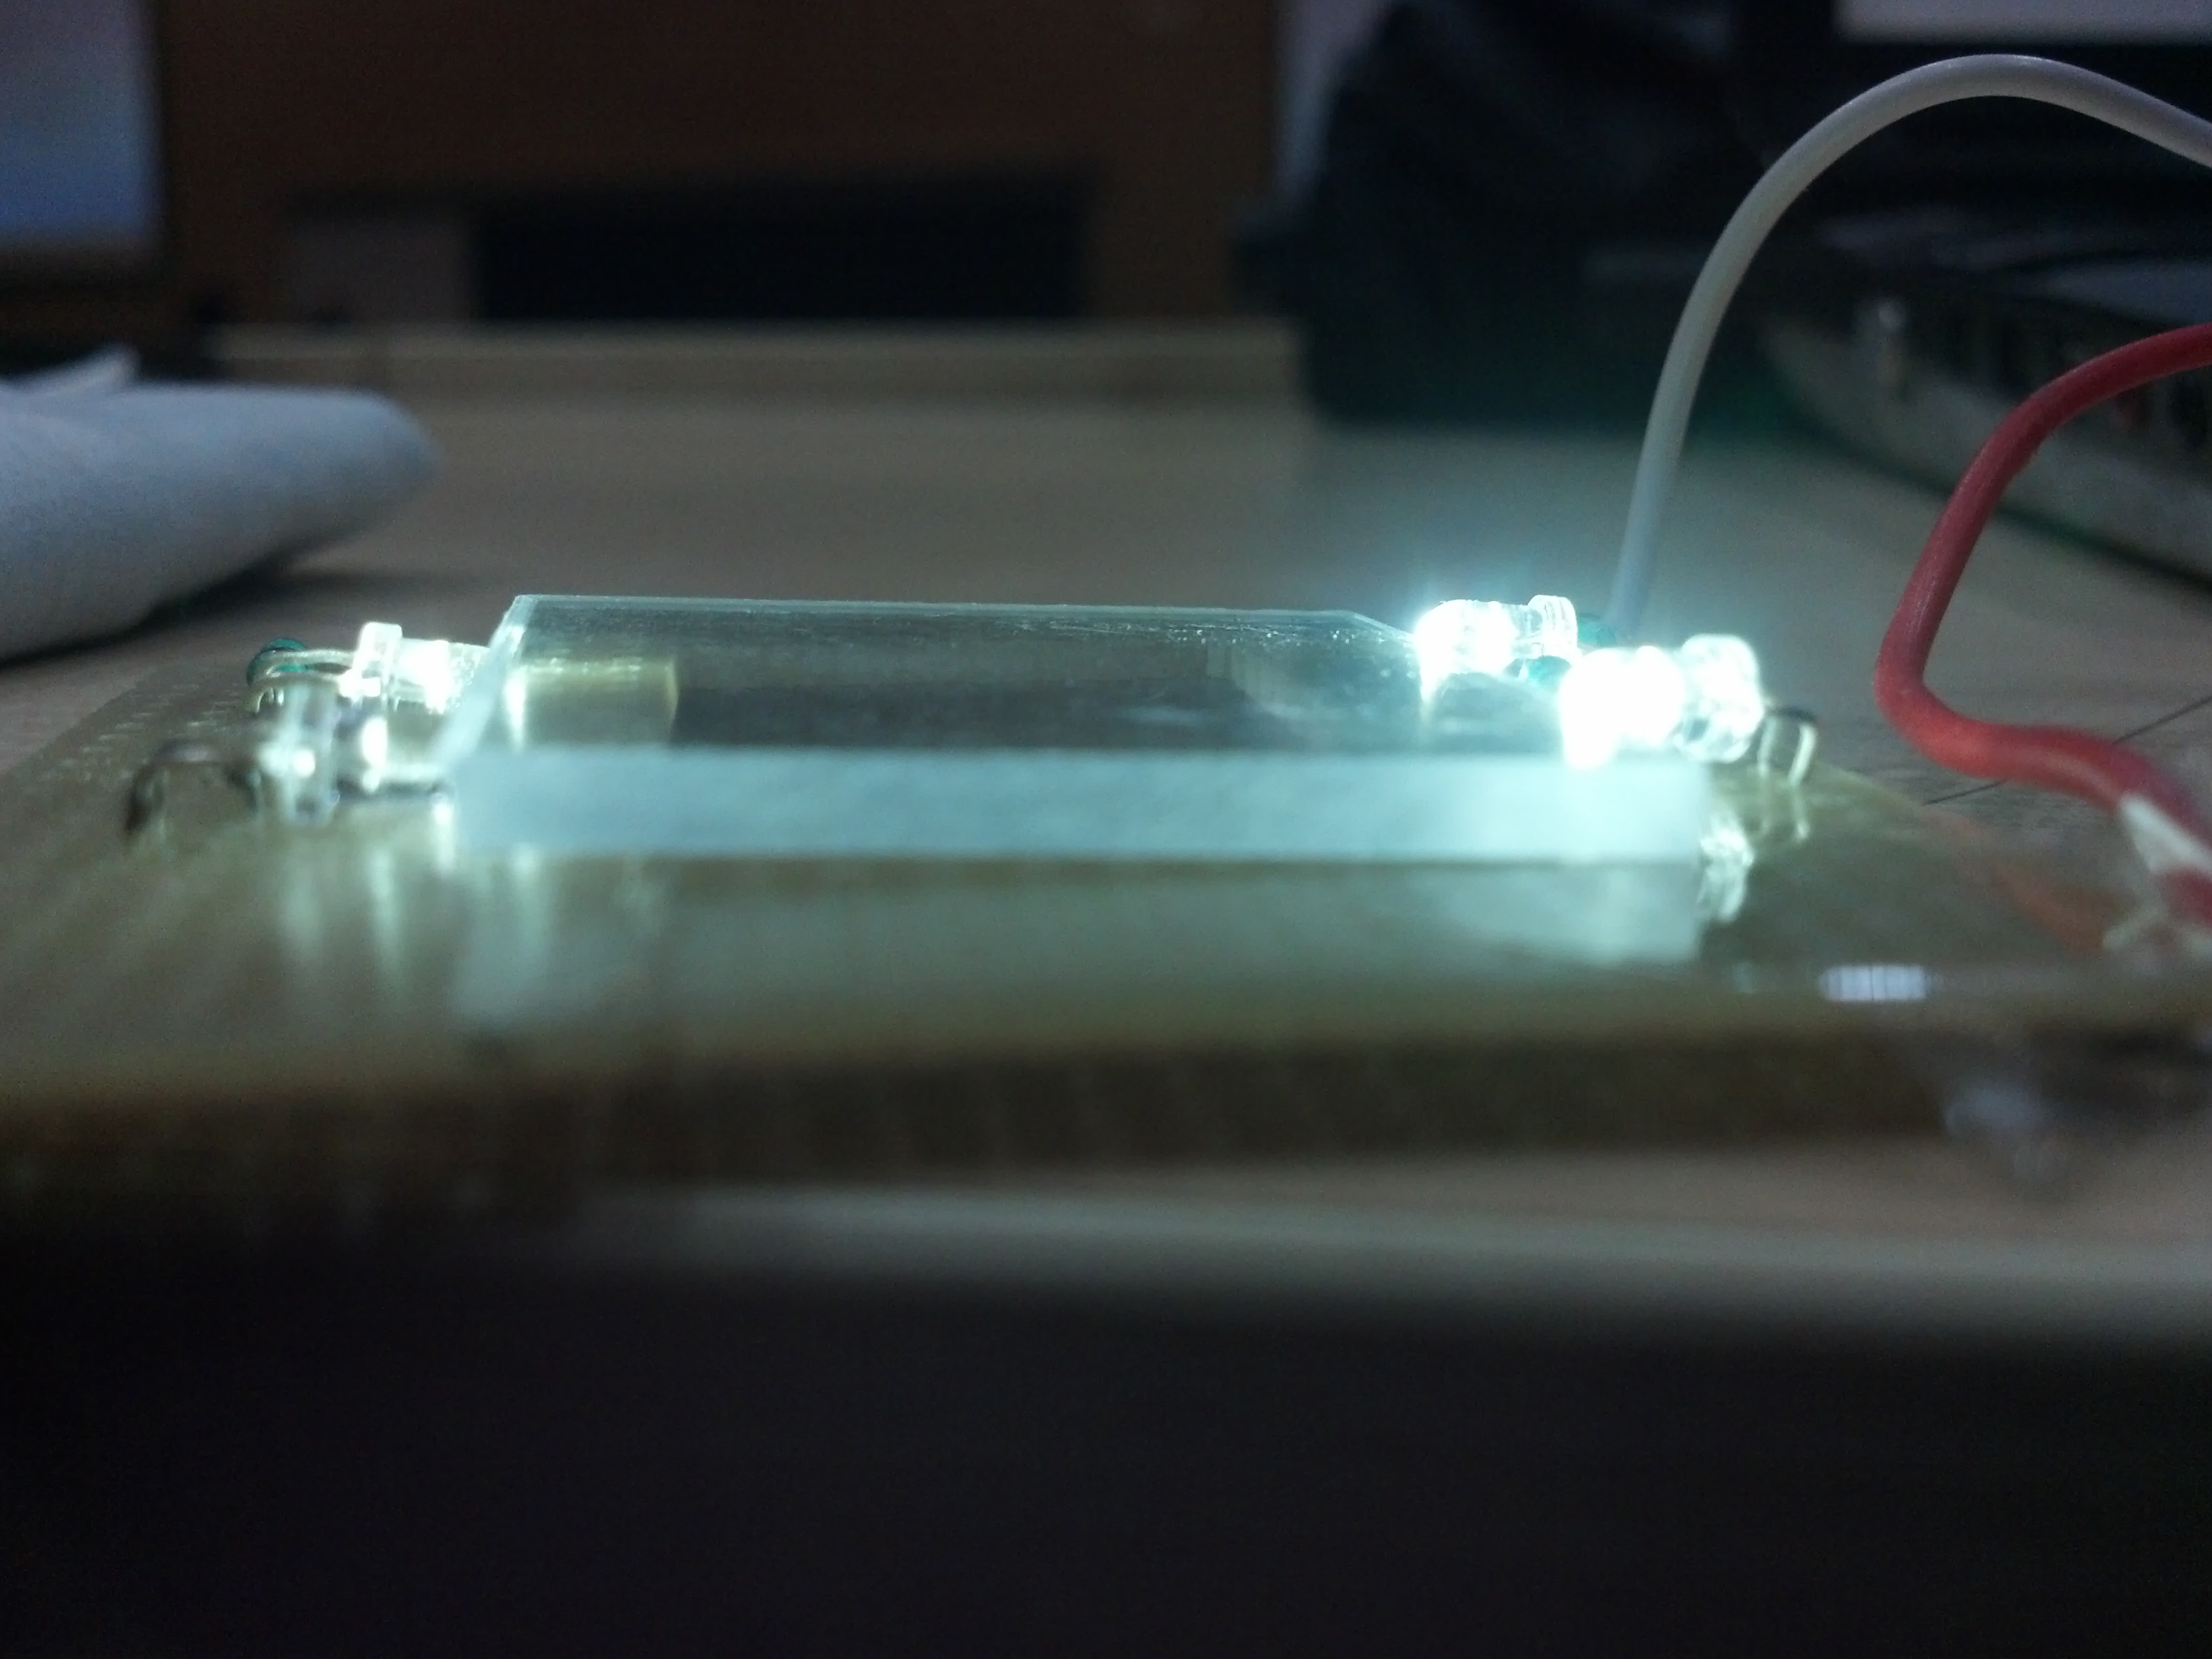
\includegraphics[width=3.5cm]{./sv.jpg}
 \caption{3.Side View}
\end{figure}
\begin{figure}
 \centering
 \vskip-20pt
 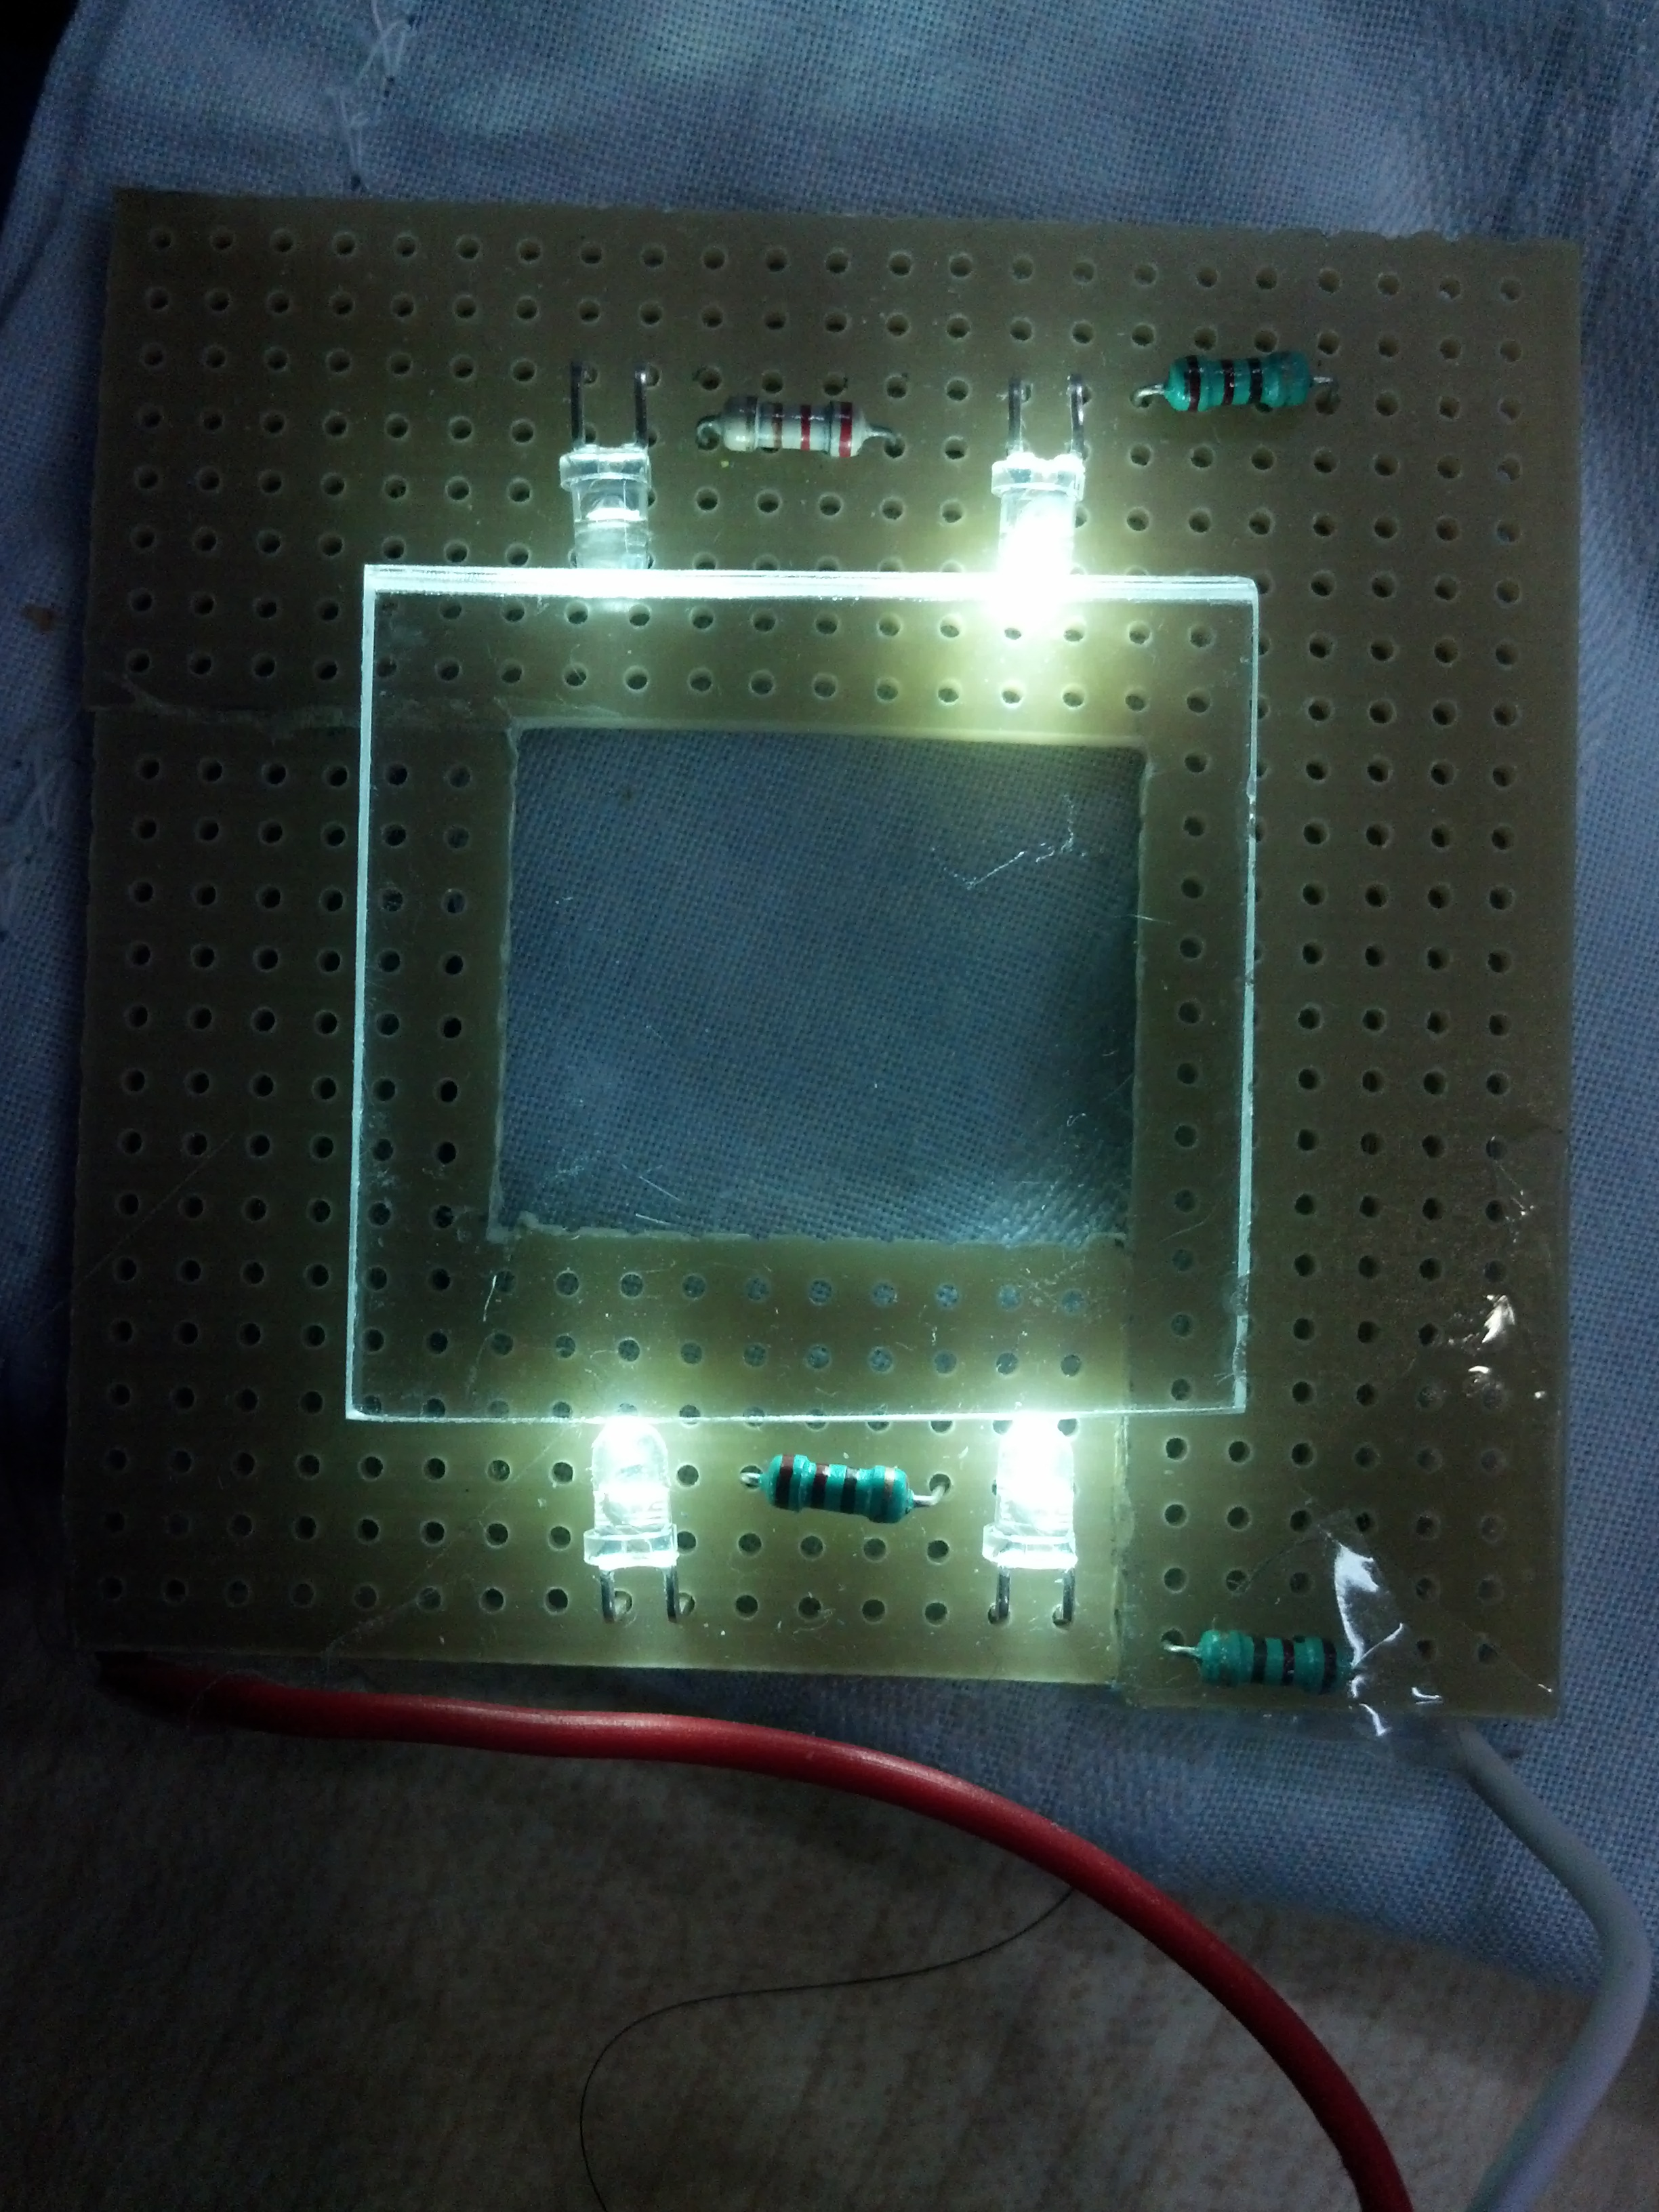
\includegraphics[width=2.5cm]{./tp.jpg}
 \caption{4.Top View}
\end{figure}
\end{frame}


\section{Hardware Used}
\begin{frame}[c]
\frametitle{Hardware Used}
\begin{enumerate}
\item \vskip-20pt Black acrylic (3 mm thick)
\item Transparent acrylic (3 mm thick, 32.5mm x 35 mm)
\item PCB
\item LEDs (4 quantity, 3 mm thick)
\item Resistors (4 quantity, 220 ohms) 
\item Power source – 4.5 V ( 3 AAA (1.5 V) cells in series)
\item Switch
\end{enumerate}
\end{frame}



\section{Frustrated Total Internal Reflection-FTIR}
\begin{frame}[c]
\frametitle{Frustrated Total Internal Reflection-FTIR}
\begin{enumerate}
 \item The behaviour of light after it hits the fingerprint ridges makes it possible to distinguish the contrast between the ridges and valleys in the image.
\end{enumerate}
\begin{figure}
 \centering
 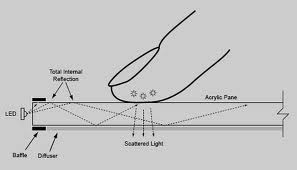
\includegraphics[width=8.5cm]{./ftir.jpg}
 \caption{5.FTIR}
\end{figure}
\end{frame}




\section{Workflow}
\begin{frame}[c]
\frametitle{Workflow}
\begin{figure}
 \centering
 \vskip-20pt
 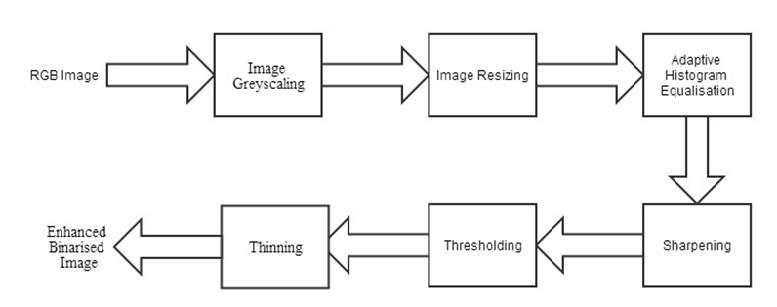
\includegraphics[width=12cm]{./wf.jpg}
 \caption{6.Workflow diagram}
\end{figure}
% \begin{enumerate}
% \item \vskip-10pt Image Capture
% \item Image Grayscaling
% \item Live Finger Detection
% \item Image Cropping
% \item Image Resizing 
% \item Adaptive Histogram Equalization
% \item Image Sharpening
% \item Image Thresholding
% \item Image Thinning
% \item Binary Image sent to server
% \end{enumerate}
\end{frame}

%--------------------------------------------------------------------------------------
%               Slide 7
%--------------------------------------------------------------------------------------
\section{Live Finger Detection}
\begin{frame}[c]
\frametitle{Live Finger Detection}
\begin{enumerate}
\item \vskip-60pt This detects whether the finger is real or a spoof.
\item The perspiration phenomenon affects the grayscale of an image. The LFD algorithm makes use of this principle.
\end{enumerate}
\end{frame}




\section{Adaptive Histogram Equalization}
\begin{frame}[c]
\frametitle{Adaptive Histogram Equalization}
\begin{enumerate}
\item \vskip-30pt It enhances the contrast of an image.
\item This makes it easier to differentiate between the parts of the image.
\item The distribution of the pixel intensities is skewed towards both the low intensity and high intensity extremes of the intensity range.
\end{enumerate}
\end{frame}


\subsection{}
\begin{frame}[c]
\frametitle{}
Algorithm:\\[12pt]
\begin{enumerate}
\item Compute the histogram.
\item Calculate normalized sum (CDF) of the histogram.
\item Transform input image to output image, using S = T(R) =CDF
\end{enumerate}
\begin{figure}
 \centering
 
 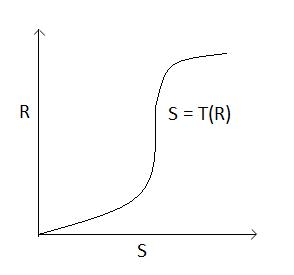
\includegraphics[width=3cm]{./ah.jpg}
 \caption{Graph}
\end{figure}
\end{frame}



\subsection{}
\begin{frame}[c]
\frametitle{}
Thus, histogram equalization helps obtain a more uniform histogram.\\
\begin{columns}[t]
\column{0.45\textwidth}
 \begin{figure}
 \centering
 \vskip-15pt
 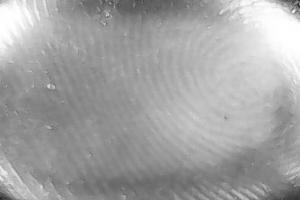
\includegraphics[width=4cm]{./ah1.jpg}
 \vskip-10pt
 \caption{Before AHE}
\end{figure}
 \begin{figure}
 \centering
 \vskip-24pt
 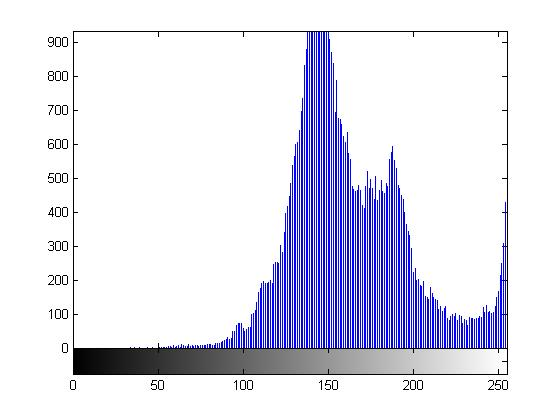
\includegraphics[width=4cm]{./ah3.jpg}
 \vskip-10pt
 \caption{Before AHE}
\end{figure}
\column{0.45\textwidth}
 \begin{figure}
 \centering
 \vskip-15pt
 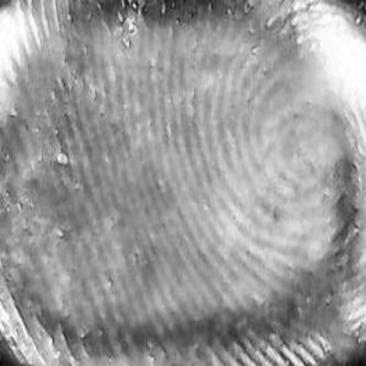
\includegraphics[width=2.8cm]{./ah2.jpg}
 \vskip-10pt
 \caption{After AHE}
\end{figure}
 \begin{figure}
 \centering
 \vskip-24pt
 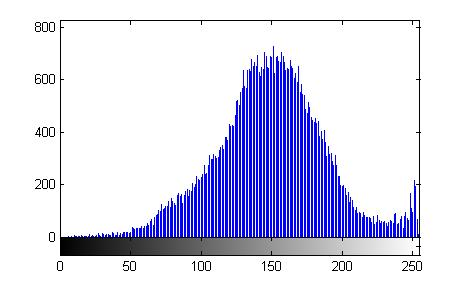
\includegraphics[width=4.6cm]{./ah4.jpg}
 \vskip-10pt
 \caption{After AHE}
\end{figure}
\end{columns}
\end{frame}

\section{Image Thresholding}
\begin{frame}[c]
\frametitle{Image Thresholding}
Thresholding is done to convert the grayscale image to a black and white image.\\[8pt]
Algorithm:
\begin{enumerate}
\item Compute the histogram and probabilities of each intensity level.
\item Set up initial probabilities and mean.
\item Step through all possible thresholds t=1…..maximum intensity.
\begin{itemize}
\footnotesize \item Update weight and mean.
\footnotesize \item Compute variance.
\footnotesize \item Compute within class  variance.
\end{itemize}
\item Desired threshold corresponds to the minimum within class variance.
\end{enumerate}
\end{frame}


\subsection{}
\begin{frame}[c]
\frametitle{}
\begin{columns}[t]
\column{0.45\textwidth}
 \begin{figure}
 \centering
 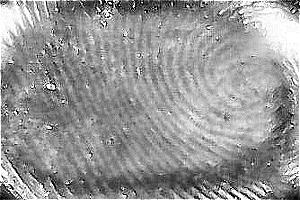
\includegraphics[width=4cm]{./th22.jpg}
 \vskip-10pt
 \caption{Before Thresholding}
\end{figure}
 \begin{figure}
 \centering
 \vskip-20pt
 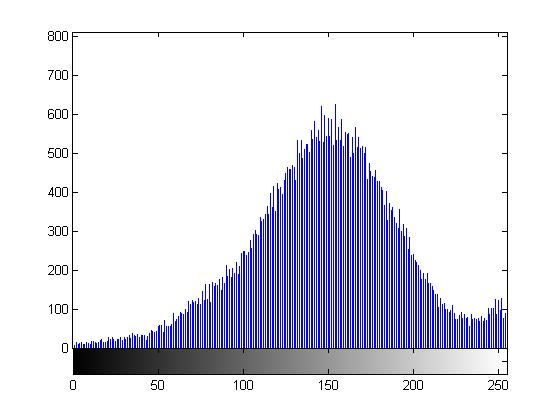
\includegraphics[width=4cm]{./th24.jpg}
 \vskip-10pt
 \caption{Before Thresholding}
\end{figure}
\column{0.45\textwidth}
 \begin{figure}
 \centering
 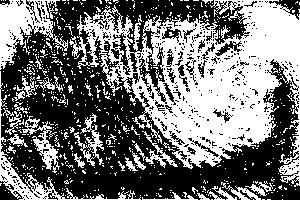
\includegraphics[width=4cm]{./th23.jpg}
 \vskip-10pt
 \caption{After Thresholding}
\end{figure}
 \begin{figure}
 \centering
 \vskip-20pt
 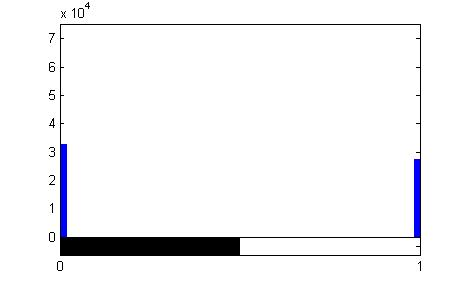
\includegraphics[width=4.5cm]{./th25.jpg}
 \vskip-10pt
 \caption{After Thresholding}
\end{figure}
\end{columns}
\end{frame}



\section{Image Sharpening}
\begin{frame}[c]
\frametitle{Image Sharpening}
\begin{enumerate}
\item \vskip-30pt Sharpening brings out image details that were not clearly visible before.
\item It enhances the pre-existing features.
\item No new details are actually created.
\item Sharpening emphasizes the edges in the image and makes it easier for the eye to pick out . 
\end{enumerate}
\end{frame}


\subsection{}
\begin{frame}[c]
\frametitle{}
\vskip-30pt
Sharpening involves the following steps:\\
\begin{enumerate}
\item Read the input image.
\item Choose the appropriate kernel to do the sharpening.
\item Apply the above kernel to the image matrix using convolution.
\item The image thus obtained, is sharpened.
\end{enumerate}
\end{frame}


\subsection{}
\begin{frame}[c]
\frametitle{}
\begin{columns}[t]
\column{0.45\textwidth}
 \begin{figure}
 \centering
 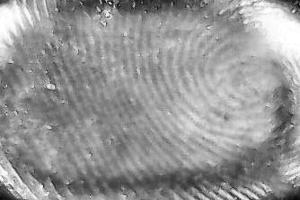
\includegraphics[width=4cm]{./sh1.jpg}
 \vskip-10pt
 \caption{Before Sharpening}
\end{figure}
 \begin{figure}
 \centering
 \vskip-20pt
 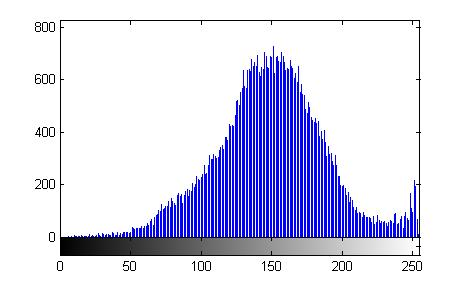
\includegraphics[width=4cm]{./sh3.jpg}
 \vskip-10pt
 \caption{Before Sharpening}
\end{figure}
\column{0.45\textwidth}
 \begin{figure}
 \centering
 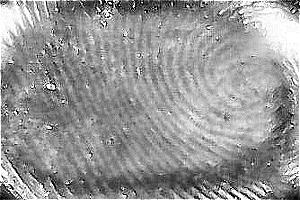
\includegraphics[width=4cm]{./sh2.jpg}
 \vskip-10pt
 \caption{After Sharpening}
\end{figure}
 \begin{figure}
 \centering
 \vskip-20pt
 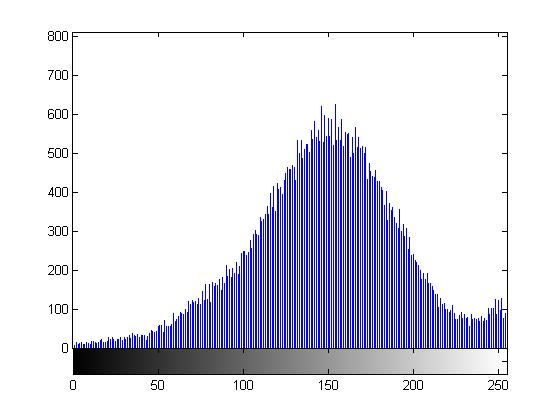
\includegraphics[width=3.2cm]{./sh4.jpg}
 \vskip-10pt
 \caption{After Sharpening}
\end{figure}
\end{columns}

\end{frame}

\section{Image Thinning}
\begin{frame}[c]
\frametitle{Image Thinning}
\begin{enumerate}
\item \vskip-30pt In thinning, the ridge lines of the fingerprint image are transformed to a one pixel thickness.
\item Thinned images require lesser memory and are easier to process. 
\item It is easier to extract details from thinned images(minutiae points) which are used for fingerprint classification, recognition and matching. 
\end{enumerate}
\end{frame}

\subsection{}
\begin{frame}[c]
\frametitle{}
Thinning can be done iteratively by deleting the pixels till they are one pixel thick.\\
\begin{figure}
 \centering
 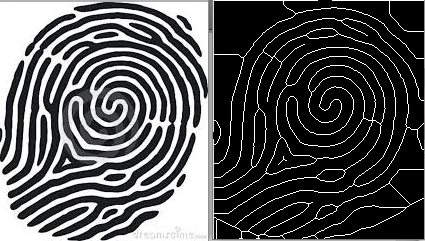
\includegraphics[width=8cm]{./thin.jpg}
 \caption{Original fingerprint image and Corresponding thinned image. }
\end{figure}
\end{frame}



\section{Future Scope}
\begin{frame}[c]
\frametitle{Future Scope}
\begin{enumerate}
\item \vskip-30pt Test the optical assembly with IR(infra-red) and SMD(Surface Mounted Device) LEDs.
\item Try different techniques like use of polarising filters and macro lenses in orded to enhance the quality of the image captured.
\item Test the enhanced image with the Aadhaar Server.
\end{enumerate}
\end{frame}


\section{Problems Faced}
\begin{frame}[c]
\frametitle{Problems faced}
\begin{enumerate}
\item \vskip-30pt Finding the distance at which the image is focused and clear.
\item Green tint in glass.
\item Illumination of the acrylic sheet.
\item Deciding workflow of image enhancement processes.
\item Implementation on Aakash tablet.
\end{enumerate}
\end{frame}

\section{Things learnt in the project}
\begin{frame}[c]
\frametitle{Things learnt in the project}
\begin{enumerate}
\item \vskip-30pt Image Processing using OpenCV.
\item Image Processing using Scilab.
\item Some algorithms used in image enhancement.
\item Developing applications on the Android platform
\item Creating a hardware assembly and overcoming various problems while doing the same.
\item Formal documentation of project(SRS, SDD and project report were submitted)
\end{enumerate}
\end{frame}


\section{Educational Application}
\begin{frame}[c]
\frametitle{Educational Application - I}
\begin{block}{Aakash Dictionary}
 \begin{columns}[c]
  \column{0.41\textwidth}
   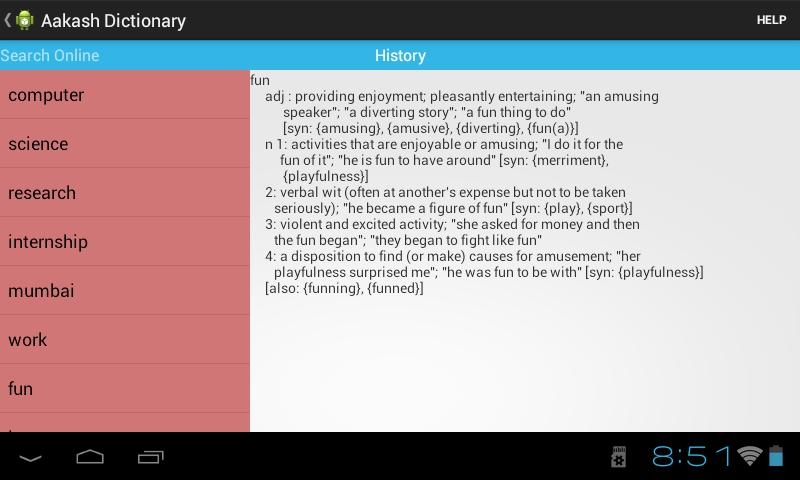
\includegraphics[width=5.5cm]{./app3.jpg}
  \column{0.50\textwidth}
  \begin{enumerate}
   \item \vskip-20pt The user can search for any word online
   \item Maintain a history of his searches
   \item He can delete any of his search.
   \end{enumerate} 
 \end{columns}
\end{block}
\end{frame}

\begin{frame}[c]
\frametitle{Educational Application - II}
\begin{block}{MathHelp!}
 \begin{columns}[c]
  \column{0.25\textwidth}
   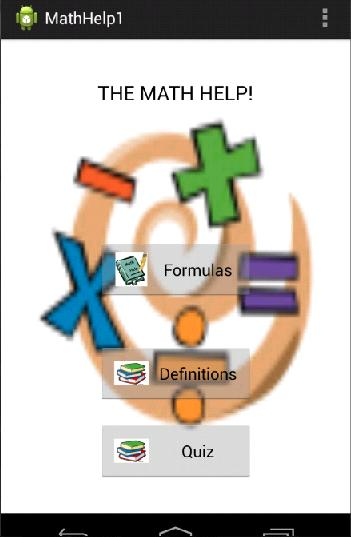
\includegraphics[width=4cm]{./app2.jpg}
  \column{0.60\textwidth}
  \begin{enumerate}
  \item \vskip-35pt Provides users with some of the basic formulas and definitions present in Algebra and Geometry.
  \item Contains a quiz that will help to revise some of the concepts in math.
 \end{enumerate}
 \end{columns}
\end{block}
\end{frame}


\begin{frame}[c]
\frametitle{Educational Application - III}
\begin{block}{Indian History}
 \begin{columns}[c]
  \column{0.34\textwidth}
   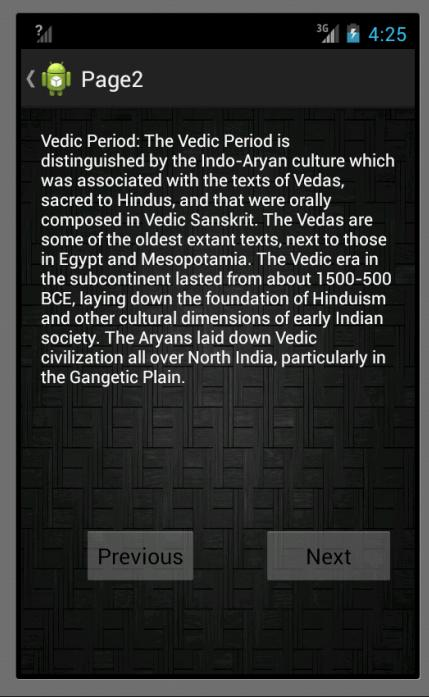
\includegraphics[width=4.5cm]{./app4.jpg}
  \column{0.62\textwidth}
  \begin{enumerate}
  \item \vskip-20pt Gives information on Indian History from Vedic era to recent years. 
  \item Contains competitive quizzes about the history of India.
 \end{enumerate}
 \end{columns}
\end{block}
\end{frame}

\begin{frame}[c]
\frametitle{Educational Application - IV}
\begin{block}{Plot Graph}
 \begin{columns}[c]
  \column{0.38\textwidth}
   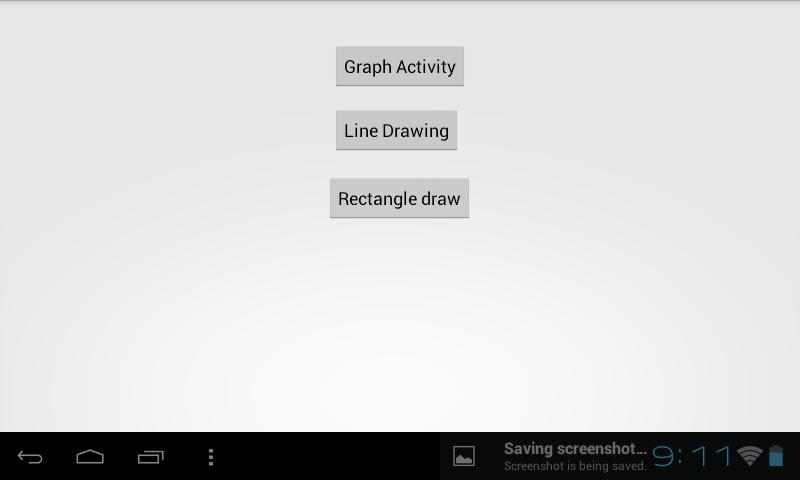
\includegraphics[width=5cm]{./app5.jpg}
  \column{0.60\textwidth}
  \begin{enumerate}
  \item \vskip-15pt Plots a line by taking the equation of the line as input.
  \item If user wants to draw a rectangle on the graph,the user needs to give the starting point and the dimensions of the rectangle. 
 
 \end{enumerate}
 \end{columns}
\end{block}
\end{frame}

\begin{frame}[c]
\frametitle{Educational Application - V}
\begin{block}{Incredible India}
 \begin{columns}[c]
  \column{0.30\textwidth}
   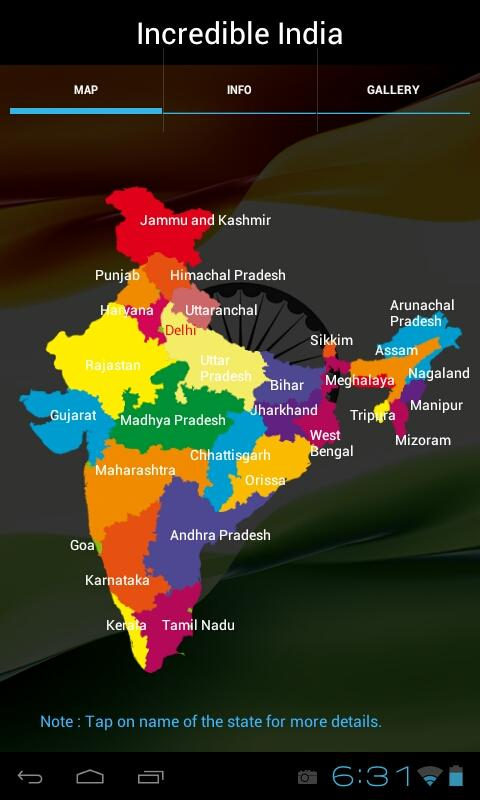
\includegraphics[width=4cm]{./app6.jpg}
  \column{0.60\textwidth}
  \begin{enumerate}
  \item \vskip-15pt On clicking on a State, a dialog box pops up with details about a particular State such as the currency,Capital and the languages spoken. 
 \end{enumerate}
 \end{columns}
\end{block}
\end{frame}


\begin{frame}[c]
\frametitle{Educational Application - VI}
\begin{block}{Periodic Table}
 \begin{columns}[c]
  \column{0.40\textwidth}
   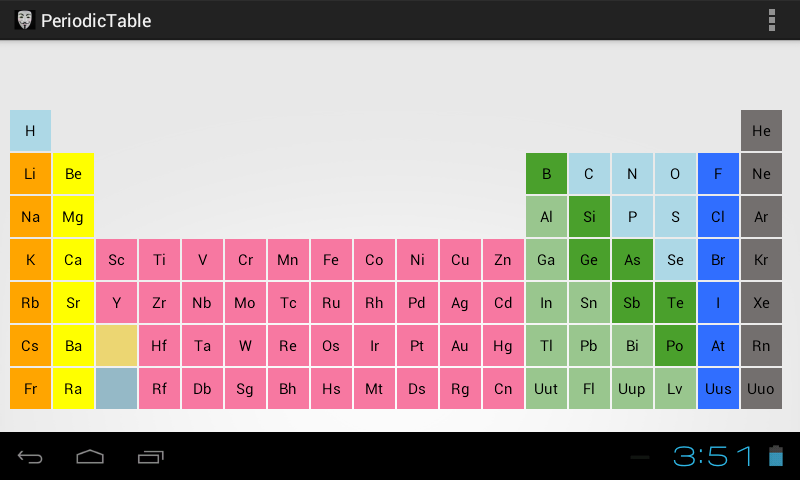
\includegraphics[width=5cm]{./app7.jpg}
  \column{0.50\textwidth}
  \begin{enumerate}
 \item \vskip-5pt Helps to understand the periodic table in detail.
 \item Gives brief information about each element and shows to which group and period it belongs.
\end{enumerate}.
 \end{columns}
\end{block}
\end{frame}



\begin{frame}[c]
\frametitle{Educational Application - VII}
\begin{block}{Consumer Protection Right}
 \begin{columns}[c]
  \column{0.42\textwidth}
   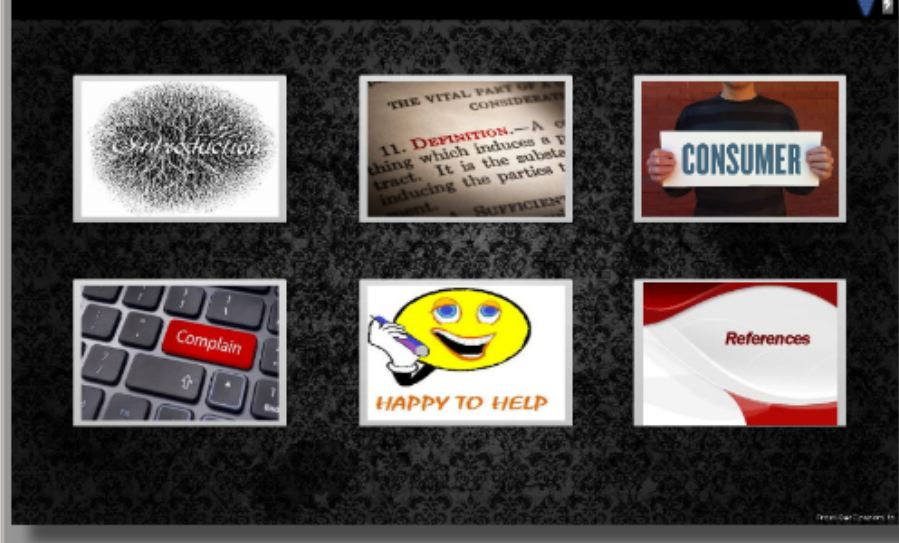
\includegraphics[width=6cm]{./app8.jpg}
  \column{0.45\textwidth}
  \begin{enumerate}
   \item \vskip-20pt Informative application which is useful for consumer to know their rights.
   \item If user faces some sort of difficulty,they can get precise guidance.
  \end{enumerate}
 \end{columns}
\end{block}
\end{frame}

\begin{frame}[c]
\frametitle{Educational Application - VIII}
\begin{block}{Salt Analysis}
 \begin{columns}[c]
  \column{0.42\textwidth}
   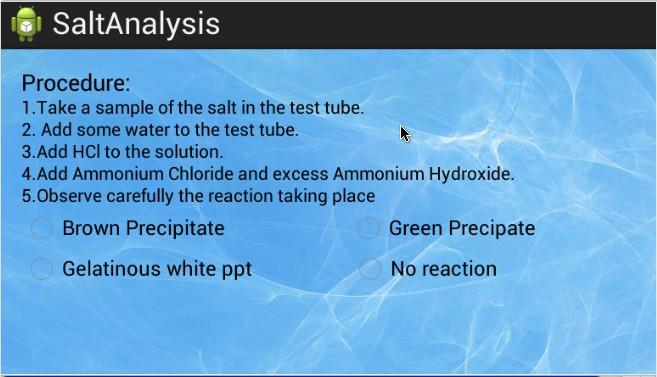
\includegraphics[width=6cm]{./h2.jpg}
  \column{0.45\textwidth}
  \begin{enumerate}
   \item \vskip-20pt Gives the user a number of steps to follow.
   \item Takes input of the result and tells the salt.
  \end{enumerate}
 \end{columns}
\end{block}
\end{frame}





\section{Demo}
\begin{frame}[c]
\frametitle{Demo}
\begin{enumerate}
\item \vskip-30pt \large DEMONSTRATION
\end{enumerate}
\end{frame}

\section{Comparison of fingerprint image}
\begin{frame}[c]
\frametitle{Comparison of fingerprint image}
Without Optical Assembly
\begin{figure}
 \centering
 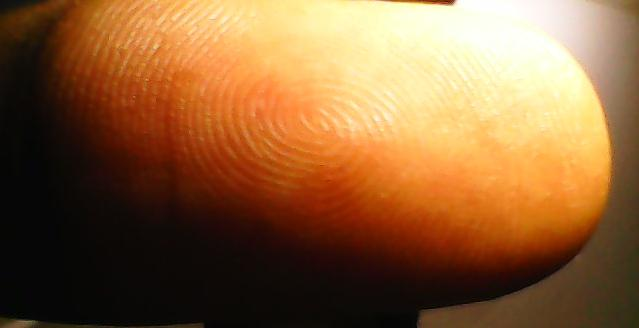
\includegraphics[width=3.5cm]{./fp.jpg}
 \caption{Fingerprint}
\end{figure}
With Optical Assembly
\begin{figure}
 \centering
 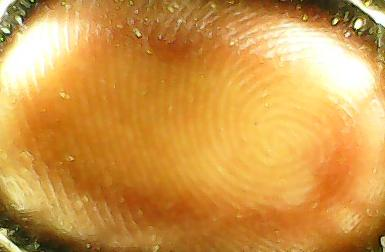
\includegraphics[width=3.5cm]{./fp1.jpg}
 \caption{Fingerprint}
\end{figure}
\end{frame}


\section{}
\begin{frame}[c]
\begin{columns}[c]
\column{0.30\textwidth}
Archana\\
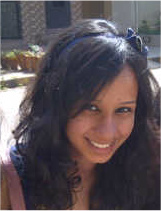
\includegraphics[width=2cm]{./arch.jpg}\\[12pt]
Hitesh\\
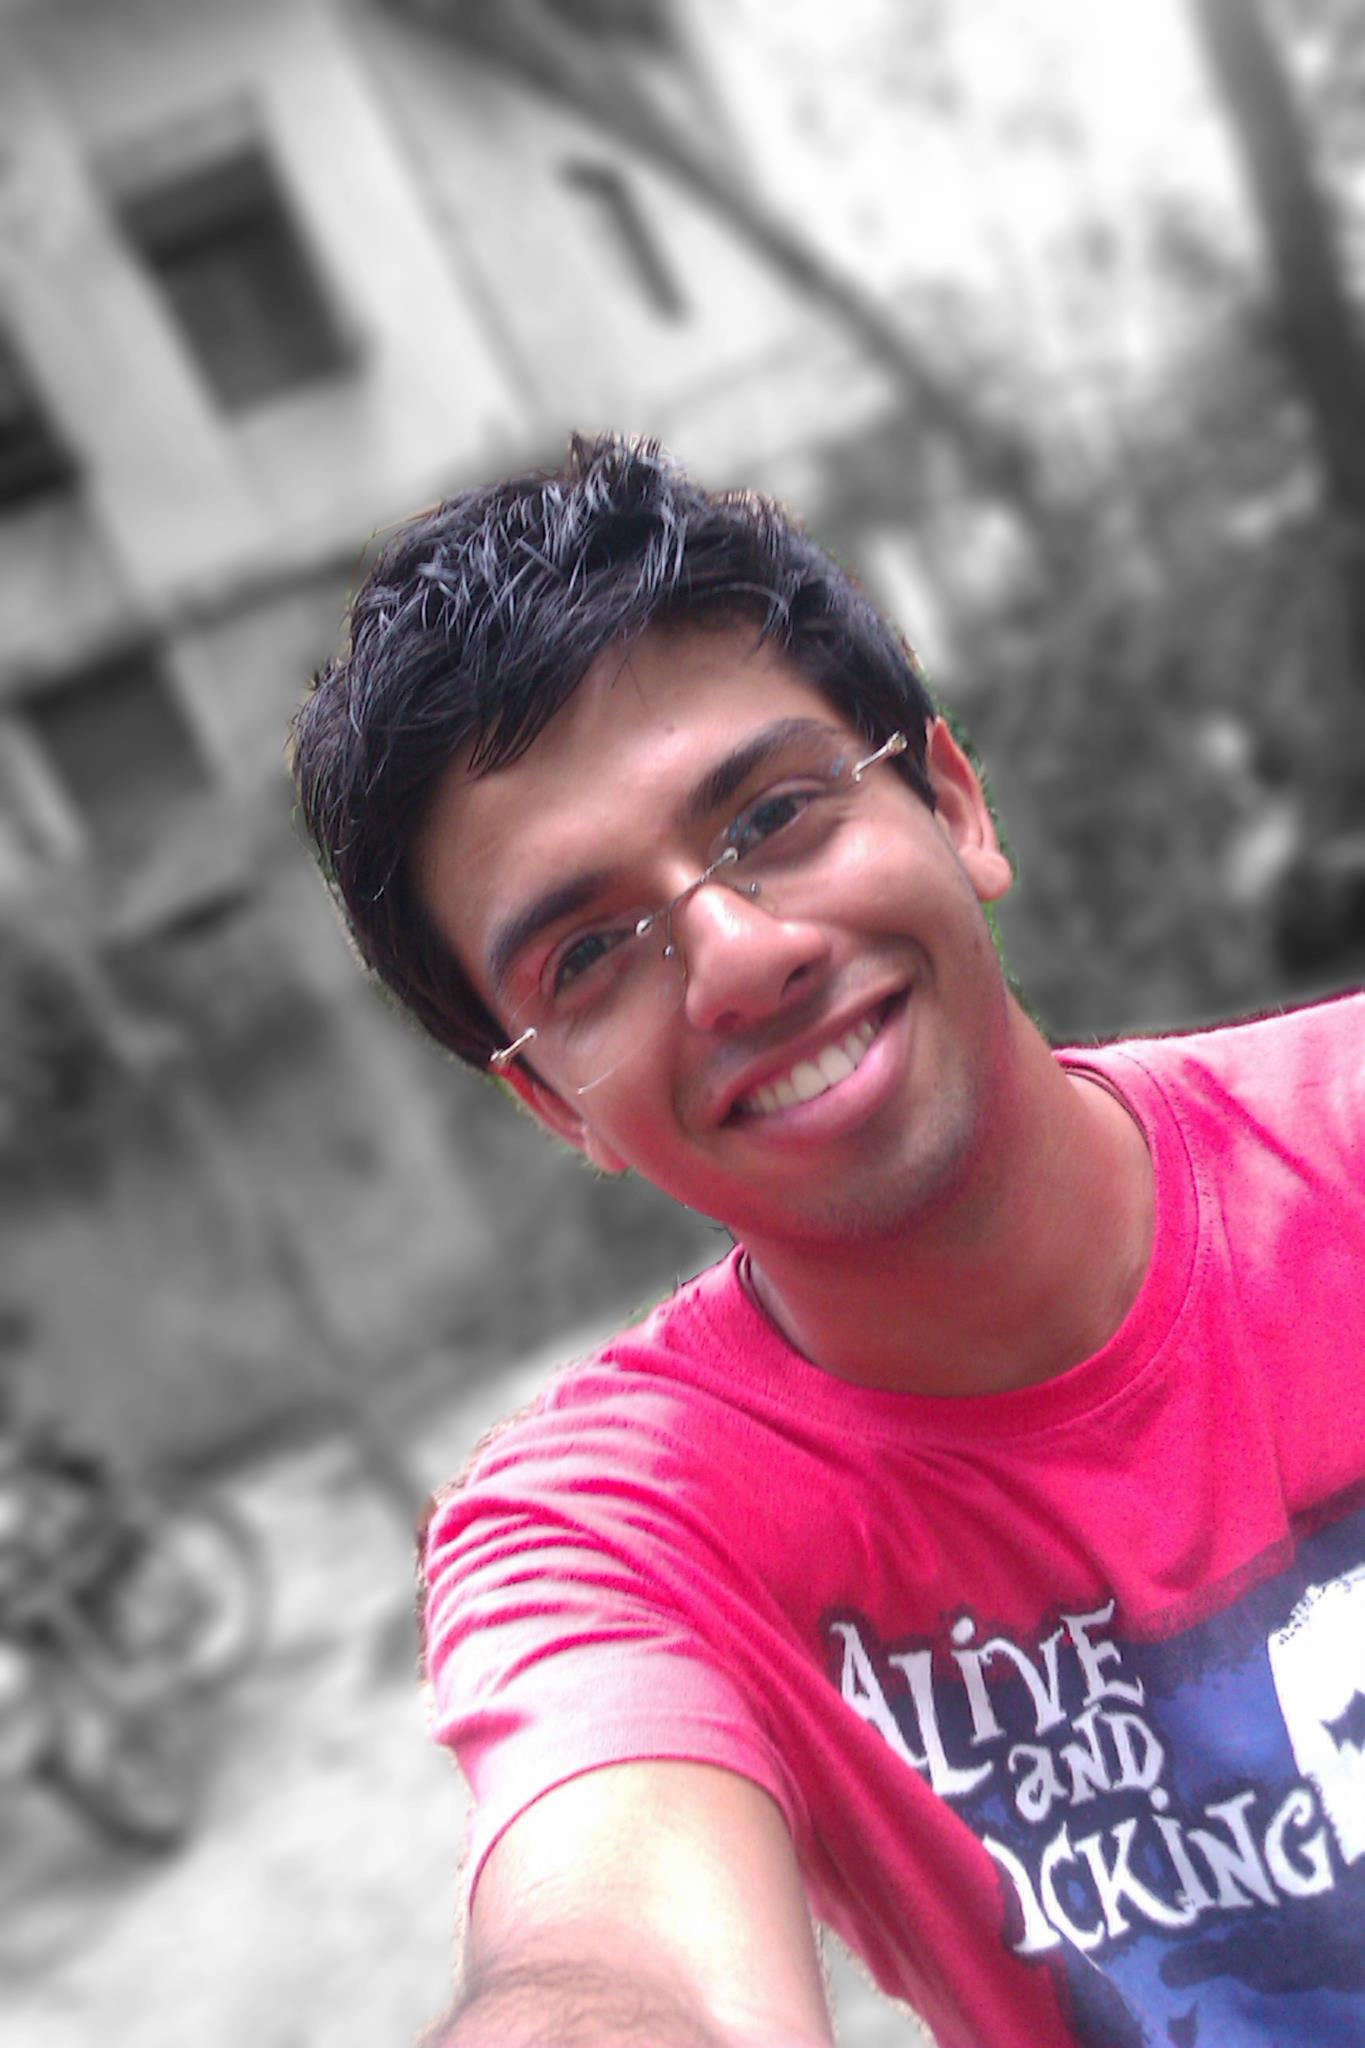
\includegraphics[width=2cm]{./h.jpg}\\
\column{0.30\textwidth}
\vskip-8pt
Pooja\\
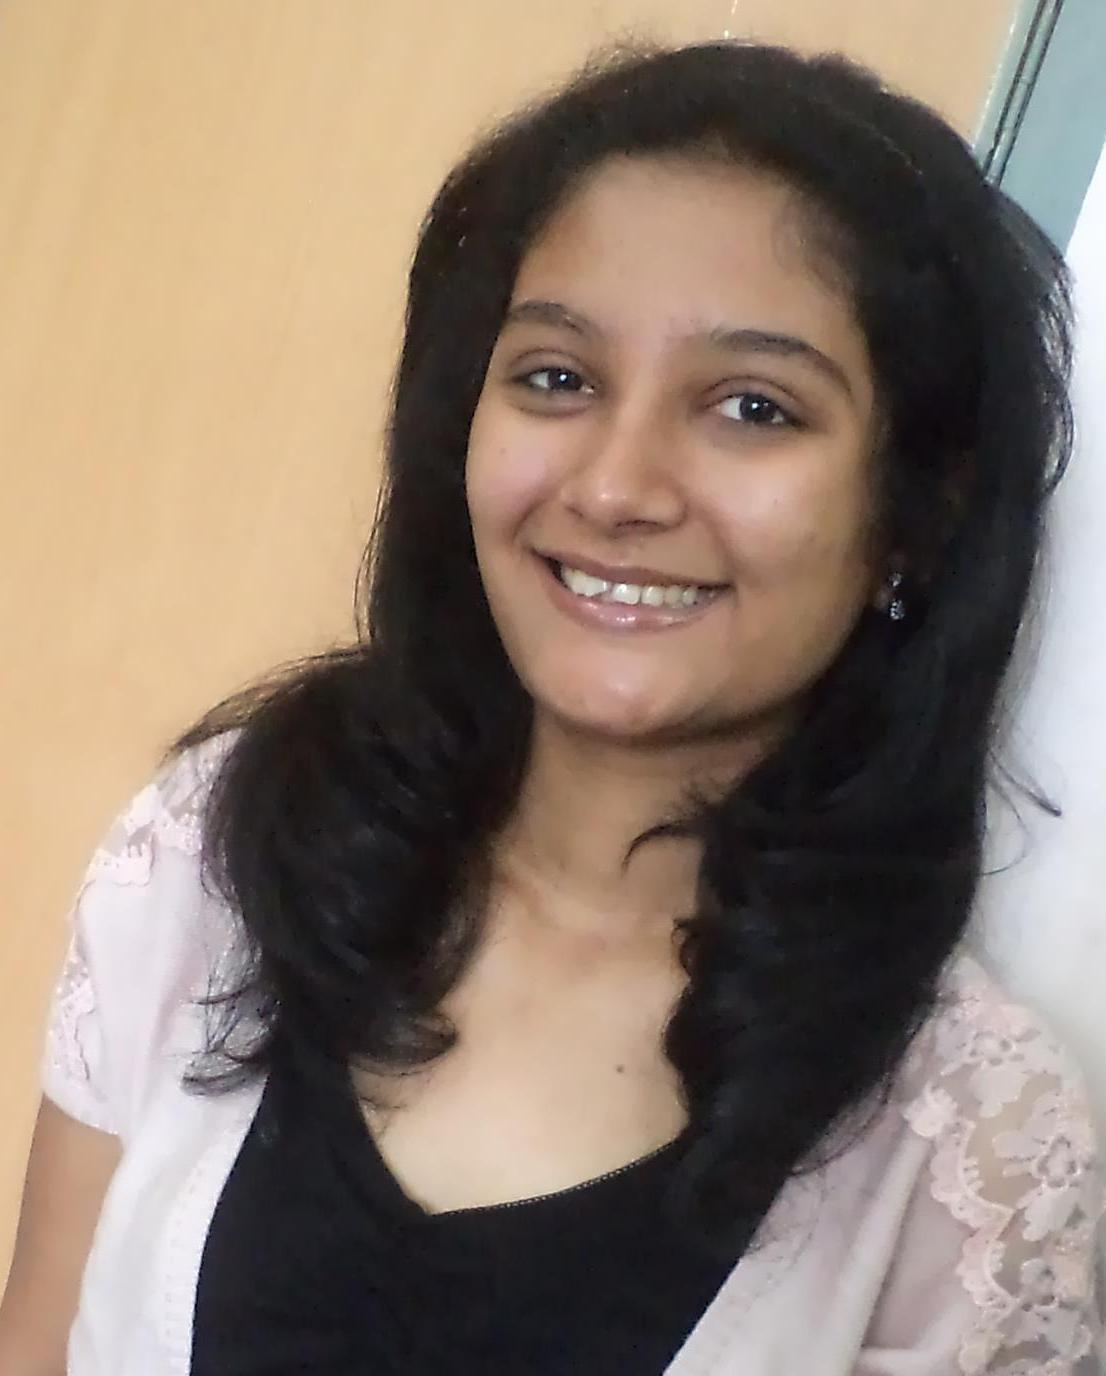
\includegraphics[width=2cm]{./poo.jpg}\\[12pt]
Prateek\\
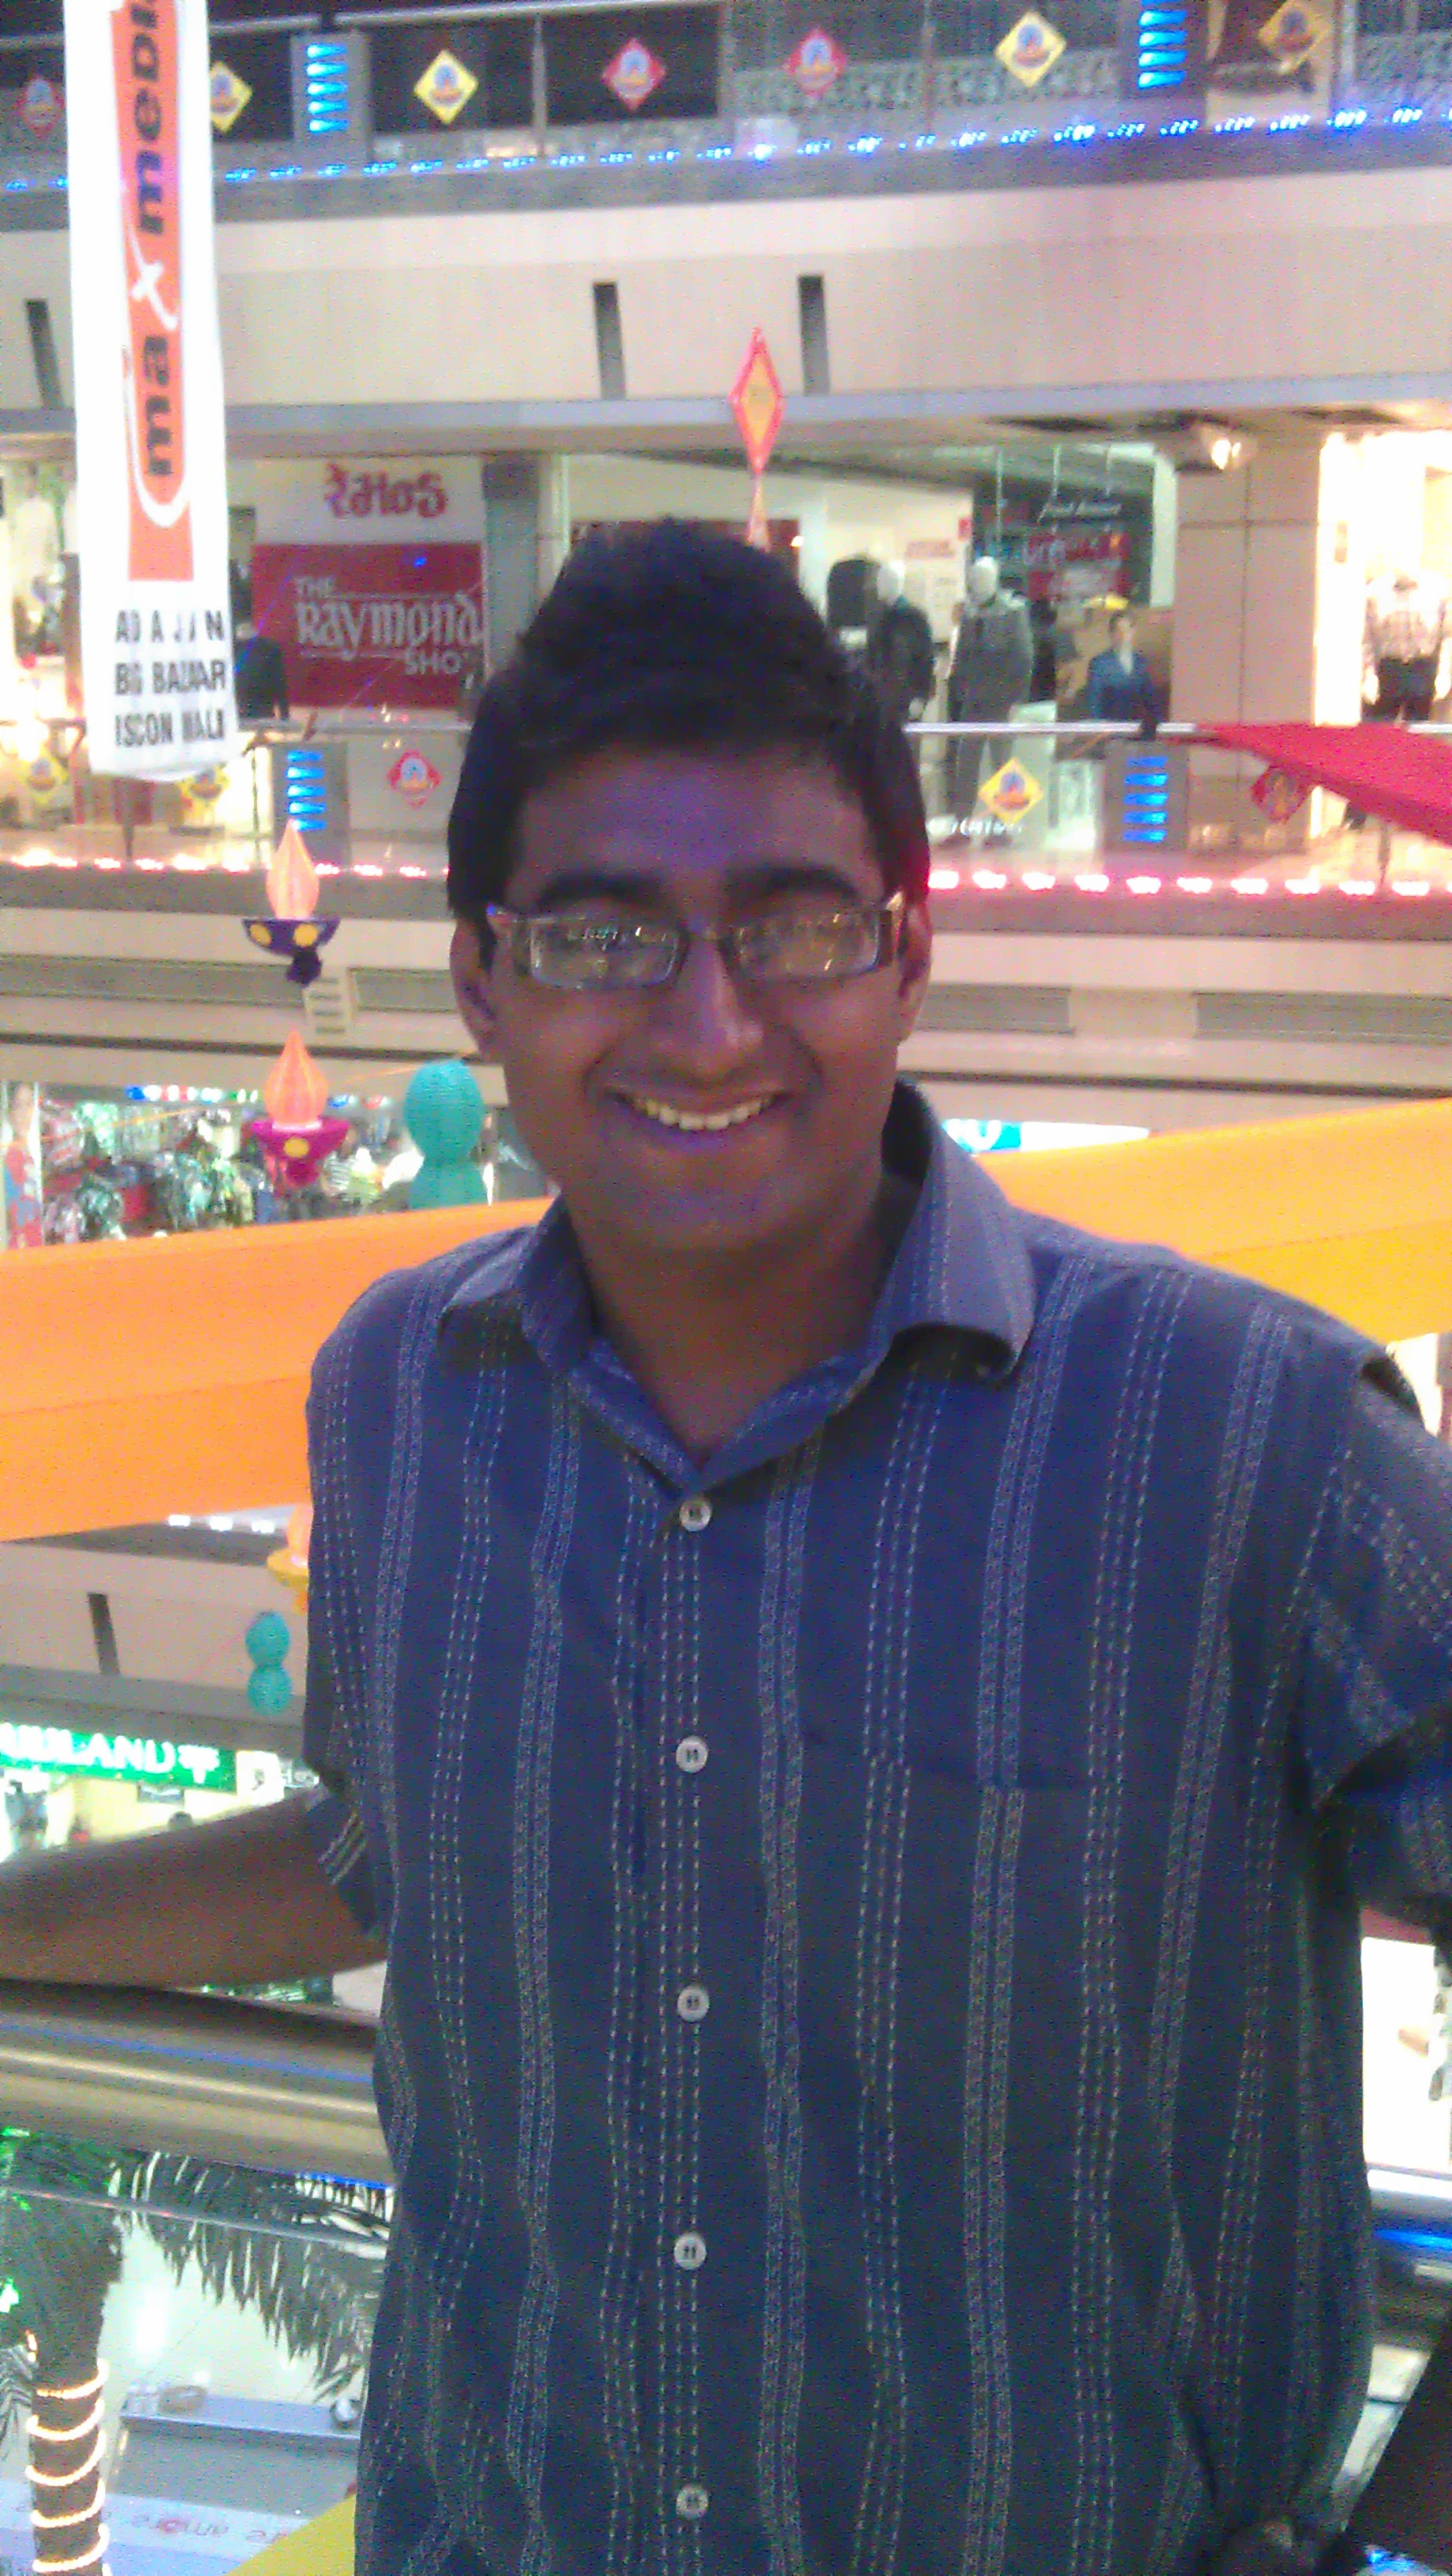
\includegraphics[width=2cm]{./pr22.jpg}\\
\column{0.30\textwidth}
Sonu\\
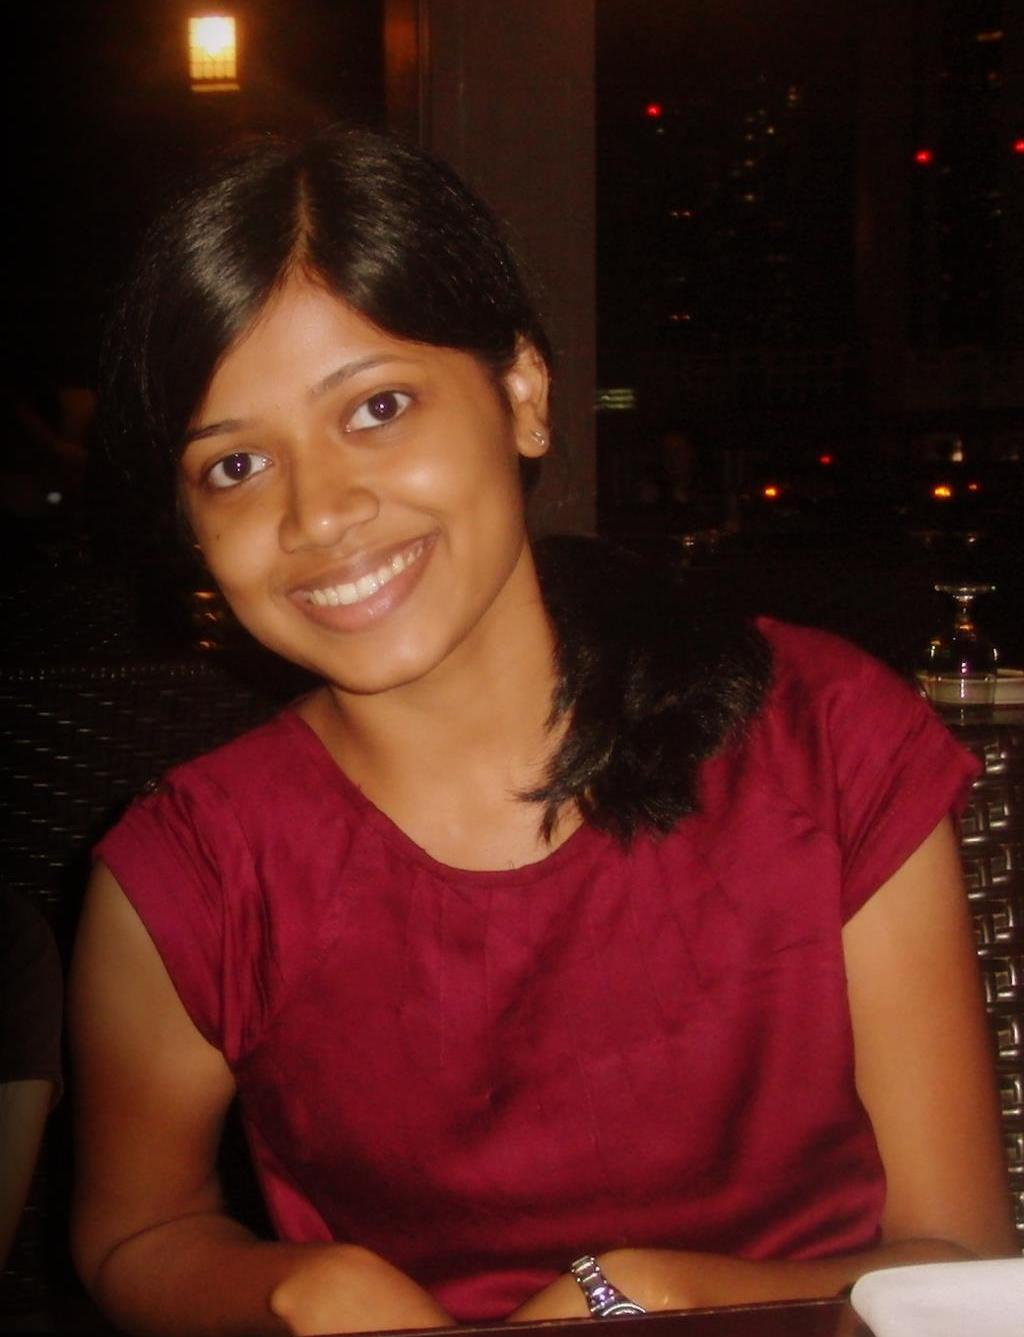
\includegraphics[width=2cm]{./sonu.jpg}\\[12pt]
Prathamesh\\
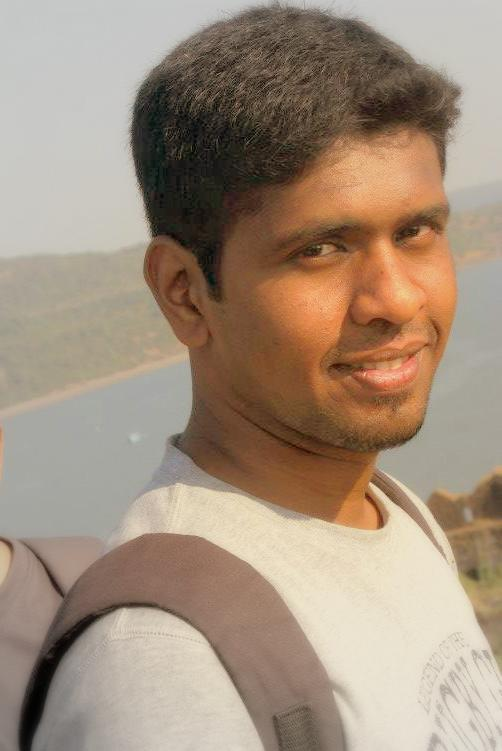
\includegraphics[width=2cm]{./prath.jpg}\\
\column{0.30\textwidth}
Prashant\\
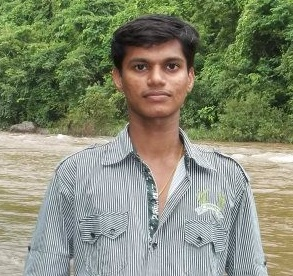
\includegraphics[width=2cm]{./pr35.jpg}\\[12pt]
Sudhanshu\\
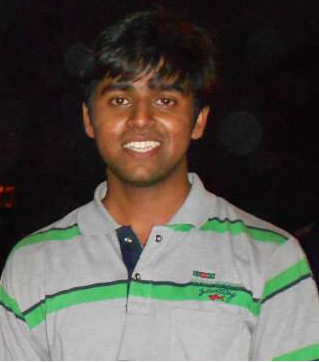
\includegraphics[width=2cm]{./sud.jpg}\\
\end{columns}
\end{frame}

\end{document}